\chapter{Basics of Convective and Radiative Heat Transfer}
This chapter explains basic aspects of convection and radiation, the two primary ways of heat transfer other than conduction. We wish to understand the concepts of buoyancy, forced convection, radiation from first principles. The hope is to establish the importance of different boundary conditions in heat 

\section{Newton's Cooling Law: When the Heat Conductor is Exposed}
\subsection{When the insulator is still there}
\quad In Lab1 we discuss the heat transfer process only by conduction, where we force thermal energy flowing at radial and axial directions by cutting off heat exchange between the conductor and ambient environment. Let's first review the setup of linear heat conduction in Lab2 (see Fig.\ref{fig1}), where we have a metal rod isolated from surrounding environment by thermal insulator. We already discussed that the temperature profile at axial direction is linear as the (1D) heat equation
\begin{marginfigure}[-2.0in]
% Gradient Info
\tikzset {_bkhwty8vx/.code = {\pgfsetadditionalshadetransform{ \pgftransformshift{\pgfpoint{0 bp } { 0 bp }  }  \pgftransformrotate{0 }  \pgftransformscale{2 }  }}}
\pgfdeclarehorizontalshading{_fmshv62bz}{150bp}{rgb(0bp)=(1,0.37,0.37);
rgb(37.5bp)=(1,0.37,0.37);
rgb(53.33928516932896bp)=(1,0.68,0.68);
rgb(62.5bp)=(1,0.68,0.68);
rgb(100bp)=(1,0.68,0.68)}
% Gradient Info
\tikzset {_ahqs6wgy5/.code = {\pgfsetadditionalshadetransform{ \pgftransformshift{\pgfpoint{0 bp } { 0 bp }  }  \pgftransformrotate{0 }  \pgftransformscale{2 }  }}}
\pgfdeclarehorizontalshading{_bkm6wwloz}{150bp}{rgb(0bp)=(0.98,0.56,0.35);
rgb(37.5bp)=(0.98,0.56,0.35);
rgb(62.5bp)=(0.98,0.71,0.61);
rgb(100bp)=(0.98,0.71,0.61)}
\tikzset{every picture/.style={line width=0.75pt}} %set default line width to 0.75pt
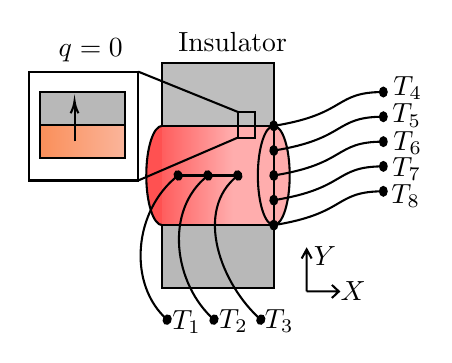
\begin{tikzpicture}[x=0.40pt,y=0.47pt,yscale=-1,xscale=0.90]
%uncomment if require: \path (0,300); %set diagram left start at 0, and has height of 300
%Shape: Ellipse [id:dp8930898544575516] 
\draw  [color={rgb, 255:red, 0; green, 0; blue, 0 }  ,draw opacity=1 ][fill={rgb, 255:red, 255; green, 81; blue, 81 }  ,fill opacity=1 ] (256,132.83) .. controls (256,111.75) and (263.16,94.67) .. (271.98,94.67) .. controls (280.81,94.67) and (287.97,111.75) .. (287.97,132.83) .. controls (287.97,153.91) and (280.81,171) .. (271.98,171) .. controls (263.16,171) and (256,153.91) .. (256,132.83) -- cycle ;
%Flowchart: Process [id:dp0921944018696561] 
\draw  [draw opacity=0][shading=_fmshv62bz,_bkhwty8vx] (271.98,94.67) -- (383.98,94.67) -- (383.98,171) -- (271.98,171) -- cycle ;
%Shape: Ellipse [id:dp01770560567207502] 
\draw  [color={rgb, 255:red, 0; green, 0; blue, 0 }  ,draw opacity=1 ][fill={rgb, 255:red, 255; green, 173; blue, 173 }  ,fill opacity=1 ] (368,132.83) .. controls (368,111.75) and (375.16,94.67) .. (383.98,94.67) .. controls (392.81,94.67) and (399.97,111.75) .. (399.97,132.83) .. controls (399.97,153.91) and (392.81,171) .. (383.98,171) .. controls (375.16,171) and (368,153.91) .. (368,132.83) -- cycle ;

%Shape: Rectangle [id:dp1097826082927833] 
\draw  [fill={rgb, 255:red, 155; green, 155; blue, 155 }  ,fill opacity=0.65 ] (271.98,46.67) -- (383.98,46.67) -- (383.98,94.67) -- (271.98,94.67) -- cycle ;
%Shape: Rectangle [id:dp46302981347640004] 
\draw  [fill={rgb, 255:red, 155; green, 155; blue, 155 }  ,fill opacity=0.71 ] (271.98,171) -- (383.98,171) -- (383.98,219) -- (271.98,219) -- cycle ;
%Straight Lines [id:da0933647333929738] 
\draw    (287.97,132.83) -- (347.97,132.83) ;
%Curve Lines [id:da2027036121237581] 
\draw    (287.97,132.83) .. controls (242.97,159.67) and (236.97,216.67) .. (276.97,243.67) ;
\draw [shift={(276.97,243.67)}, rotate = 34.02] [color={rgb, 255:red, 0; green, 0; blue, 0 }  ][fill={rgb, 255:red, 0; green, 0; blue, 0 }  ][line width=0.75]      (0, 0) circle [x radius= 3.35, y radius= 3.35]   ;
\draw [shift={(287.97,132.83)}, rotate = 149.19] [color={rgb, 255:red, 0; green, 0; blue, 0 }  ][fill={rgb, 255:red, 0; green, 0; blue, 0 }  ][line width=0.75]      (0, 0) circle [x radius= 3.35, y radius= 3.35]   ;
%Curve Lines [id:da007424260196329913] 
\draw    (317.97,132.83) .. controls (272.97,159.67) and (283.97,216.67) .. (323.97,243.67) ;
\draw [shift={(323.97,243.67)}, rotate = 34.02] [color={rgb, 255:red, 0; green, 0; blue, 0 }  ][fill={rgb, 255:red, 0; green, 0; blue, 0 }  ][line width=0.75]      (0, 0) circle [x radius= 3.35, y radius= 3.35]   ;
\draw [shift={(317.97,132.83)}, rotate = 149.19] [color={rgb, 255:red, 0; green, 0; blue, 0 }  ][fill={rgb, 255:red, 0; green, 0; blue, 0 }  ][line width=0.75]      (0, 0) circle [x radius= 3.35, y radius= 3.35]   ;
%Curve Lines [id:da6978833949752885] 
\draw    (347.97,132.83) .. controls (302.97,159.67) and (330.97,216.67) .. (370.97,243.67) ;
\draw [shift={(370.97,243.67)}, rotate = 34.02] [color={rgb, 255:red, 0; green, 0; blue, 0 }  ][fill={rgb, 255:red, 0; green, 0; blue, 0 }  ][line width=0.75]      (0, 0) circle [x radius= 3.35, y radius= 3.35]   ;
\draw [shift={(347.97,132.83)}, rotate = 149.19] [color={rgb, 255:red, 0; green, 0; blue, 0 }  ][fill={rgb, 255:red, 0; green, 0; blue, 0 }  ][line width=0.75]      (0, 0) circle [x radius= 3.35, y radius= 3.35]   ;
%Straight Lines [id:da8939128650475621] 
\draw    (383.98,94.67) -- (383.98,171) ;
%Curve Lines [id:da9227013430103824] 
\draw    (383.98,94.67) .. controls (457.97,85.67) and (443.97,68.67) .. (493.97,68.67) ;
\draw [shift={(493.97,68.67)}, rotate = 0] [color={rgb, 255:red, 0; green, 0; blue, 0 }  ][fill={rgb, 255:red, 0; green, 0; blue, 0 }  ][line width=0.75]      (0, 0) circle [x radius= 3.35, y radius= 3.35]   ;
\draw [shift={(383.98,94.67)}, rotate = 353.06] [color={rgb, 255:red, 0; green, 0; blue, 0 }  ][fill={rgb, 255:red, 0; green, 0; blue, 0 }  ][line width=0.75]      (0, 0) circle [x radius= 3.35, y radius= 3.35]   ;
%Curve Lines [id:da40665612439603094] 
\draw    (383.98,113.67) .. controls (457.97,104.67) and (443.97,87.67) .. (493.97,87.67) ;
\draw [shift={(493.97,87.67)}, rotate = 0] [color={rgb, 255:red, 0; green, 0; blue, 0 }  ][fill={rgb, 255:red, 0; green, 0; blue, 0 }  ][line width=0.75]      (0, 0) circle [x radius= 3.35, y radius= 3.35]   ;
\draw [shift={(383.98,113.67)}, rotate = 353.06] [color={rgb, 255:red, 0; green, 0; blue, 0 }  ][fill={rgb, 255:red, 0; green, 0; blue, 0 }  ][line width=0.75]      (0, 0) circle [x radius= 3.35, y radius= 3.35]   ;
%Curve Lines [id:da617260728715295] 
\draw    (383.98,132.83) .. controls (457.97,123.83) and (443.97,106.83) .. (493.97,106.83) ;
\draw [shift={(493.97,106.83)}, rotate = 0] [color={rgb, 255:red, 0; green, 0; blue, 0 }  ][fill={rgb, 255:red, 0; green, 0; blue, 0 }  ][line width=0.75]      (0, 0) circle [x radius= 3.35, y radius= 3.35]   ;
\draw [shift={(383.98,132.83)}, rotate = 353.06] [color={rgb, 255:red, 0; green, 0; blue, 0 }  ][fill={rgb, 255:red, 0; green, 0; blue, 0 }  ][line width=0.75]      (0, 0) circle [x radius= 3.35, y radius= 3.35]   ;
%Curve Lines [id:da8978148840999268] 
\draw    (383.98,151.83) .. controls (457.97,142.83) and (443.97,125.83) .. (493.97,125.83) ;
\draw [shift={(493.97,125.83)}, rotate = 0] [color={rgb, 255:red, 0; green, 0; blue, 0 }  ][fill={rgb, 255:red, 0; green, 0; blue, 0 }  ][line width=0.75]      (0, 0) circle [x radius= 3.35, y radius= 3.35]   ;
\draw [shift={(383.98,151.83)}, rotate = 353.06] [color={rgb, 255:red, 0; green, 0; blue, 0 }  ][fill={rgb, 255:red, 0; green, 0; blue, 0 }  ][line width=0.75]      (0, 0) circle [x radius= 3.35, y radius= 3.35]   ;
%Curve Lines [id:da9974584127929086] 
\draw    (383.98,171) .. controls (457.97,162) and (443.97,145) .. (493.97,145) ;
\draw [shift={(493.97,145)}, rotate = 0] [color={rgb, 255:red, 0; green, 0; blue, 0 }  ][fill={rgb, 255:red, 0; green, 0; blue, 0 }  ][line width=0.75]      (0, 0) circle [x radius= 3.35, y radius= 3.35]   ;
\draw [shift={(383.98,171)}, rotate = 353.06] [color={rgb, 255:red, 0; green, 0; blue, 0 }  ][fill={rgb, 255:red, 0; green, 0; blue, 0 }  ][line width=0.75]      (0, 0) circle [x radius= 3.35, y radius= 3.35]   ;
%Shape: Axis 2D [id:dp3638519525035724] 
\draw  (417,222) -- (449.33,222)(417,189.67) -- (417,222) -- cycle (442.33,217) -- (449.33,222) -- (442.33,227) (412,196.67) -- (417,189.67) -- (422,196.67)  ;

%Shape: Rectangle [id:dp33581614686961236] 
\draw   (348,84) -- (364.97,84) -- (364.97,103.67) -- (348,103.67) -- cycle ;
%Shape: Rectangle [id:dp1316064357820631] 
\draw  [fill={rgb, 255:red, 155; green, 155; blue, 155 }  ,fill opacity=0.71 ] (149,68.67) -- (234.97,68.67) -- (234.97,94) -- (149,94) -- cycle ;
%Shape: Rectangle [id:dp7870171144066422] 
\path  [shading=_bkm6wwloz,_ahqs6wgy5] (149,94) -- (234.97,94) -- (234.97,119.33) -- (149,119.33) -- cycle ; % for fading 
 \draw   (149,94) -- (234.97,94) -- (234.97,119.33) -- (149,119.33) -- cycle ; % for border 

%Straight Lines [id:da47888608604197413] 
\draw    (184,106.67) -- (184,77.67) ;
\draw [shift={(184,75.67)}, rotate = 450] [color={rgb, 255:red, 0; green, 0; blue, 0 }  ][line width=0.75]    (10.93,-3.29) .. controls (6.95,-1.4) and (3.31,-0.3) .. (0,0) .. controls (3.31,0.3) and (6.95,1.4) .. (10.93,3.29)   ;
%Shape: Rectangle [id:dp6318792554583743] 
\draw   (138,53) -- (247.97,53) -- (247.97,136.67) -- (138,136.67) -- cycle ;
%Straight Lines [id:da775439369445763] 
\draw    (247.97,53) -- (348,84) ;
%Straight Lines [id:da2765807872192515] 
\draw    (247.97,136.67) -- (348,103.67) ;
% Text Node
\draw (372,233.47) node [anchor=north west][inner sep=0.75pt]    {$T_{3}$};
% Text Node
\draw (326,233.47) node [anchor=north west][inner sep=0.75pt]    {$T_{2}$};
% Text Node
\draw (279,234) node [anchor=north west][inner sep=0.75pt]    {$T_{1}$};
% Text Node
\draw (499,137.47) node [anchor=north west][inner sep=0.75pt]    {$T_{8}$};
% Text Node
\draw (500,116.47) node [anchor=north west][inner sep=0.75pt]    {$T_{7}$};
% Text Node
\draw (501,96.47) node [anchor=north west][inner sep=0.75pt]    {$T_{6}$};
% Text Node
\draw (500,75.47) node [anchor=north west][inner sep=0.75pt]    {$T_{5}$};
% Text Node
\draw (501,54.47) node [anchor=north west][inner sep=0.75pt]    {$T_{4}$};
% Text Node
\draw (285,20) node [anchor=north west][inner sep=0.75pt]   [align=left] {Insulator};
% Text Node
\draw (165,25) node [anchor=north west][inner sep=0.75pt]    {$q=0$};
% Text Node
\draw (421,185) node [anchor=north west][inner sep=0.75pt]    {$Y$};
% Text Node
\draw (448,212) node [anchor=north west][inner sep=0.75pt]    {$X$};
\end{tikzpicture}
\caption{Schematic of one-dimensional conduction.}
\label{fig1}
\end{marginfigure}
$$
\frac{\partial T}{\partial t}=\alpha\frac{\partial^2T}{\partial x^2}
$$
at steady state becomes
$$
0=\alpha\frac{\partial^2T}{\partial x^2},
$$

\noindent which has a simple solution of $T=ax+b$. But \imp{\textbf{what if we want to be more realistic by considering the heat transfer along the radial direction?}} 

\begin{marginfigure}
\tikzset{every picture/.style={line width=0.75pt}} %set default line width to 0.75pt        
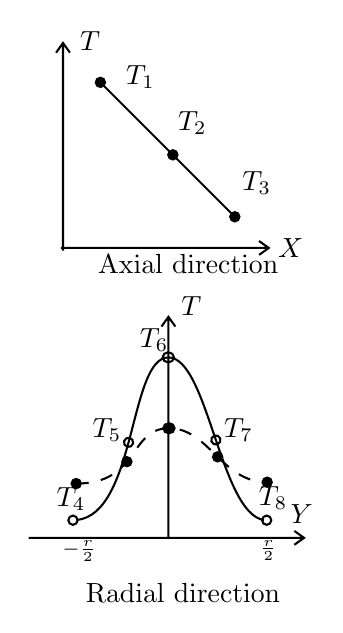
\begin{tikzpicture}[x=0.5pt,y=0.5pt,yscale=-1,xscale=1]
%uncomment if require: \path (0,461); %set diagram left start at 0, and has height of 461

%Shape: Axis 2D [id:dp7203972057491987] 
\draw  (144.33,202.46) -- (294.48,202.46)(145.78,54.32) -- (145.78,204.46) (287.48,197.46) -- (294.48,202.46) -- (287.48,207.46) (140.78,61.32) -- (145.78,54.32) -- (150.78,61.32)  ;
%Straight Lines [id:da012720486378675178] 
\draw    (225.17,135.16) -- (269.95,179.94) ;
\draw [shift={(269.95,179.94)}, rotate = 45] [color={rgb, 255:red, 0; green, 0; blue, 0 }  ][fill={rgb, 255:red, 0; green, 0; blue, 0 }  ][line width=0.75]      (0, 0) circle [x radius= 3.35, y radius= 3.35]   ;
%Straight Lines [id:da5535460113687797] 
\draw    (172.81,82.8) -- (225.17,135.16) ;
\draw [shift={(225.17,135.16)}, rotate = 45] [color={rgb, 255:red, 0; green, 0; blue, 0 }  ][fill={rgb, 255:red, 0; green, 0; blue, 0 }  ][line width=0.75]      (0, 0) circle [x radius= 3.35, y radius= 3.35]   ;
\draw [shift={(172.81,82.8)}, rotate = 45] [color={rgb, 255:red, 0; green, 0; blue, 0 }  ][fill={rgb, 255:red, 0; green, 0; blue, 0 }  ][line width=0.75]      (0, 0) circle [x radius= 3.35, y radius= 3.35]   ;
%Shape: Axis 2D [id:dp48699514611739636] 
\draw  (121,411.97) -- (319.97,411.97)(221.97,252.26) -- (221.97,411.97) (312.97,406.97) -- (319.97,411.97) -- (312.97,416.97) (216.97,259.26) -- (221.97,252.26) -- (226.97,259.26)  ;
%Curve Lines [id:da5699172388708577] 
\draw    (155.66,399.08) .. controls (198.74,394.57) and (193.55,281.59) .. (221.97,281.59) .. controls (250.39,281.59) and (259.6,394.57) .. (291.02,399.08) ;
\draw [shift={(292.97,399.22)}, rotate = 0] [color={rgb, 255:red, 0; green, 0; blue, 0 }  ][line width=0.75]      (0, 0) circle [x radius= 3.35, y radius= 3.35]   ;
\draw [shift={(193.15,342.97)}, rotate = 285.57] [color={rgb, 255:red, 0; green, 0; blue, 0 }  ][line width=0.75]      (0, 0) circle [x radius= 3.35, y radius= 3.35]   ;
\draw [shift={(256.25,341.24)}, rotate = 71.24] [color={rgb, 255:red, 0; green, 0; blue, 0 }  ][line width=0.75]      (0, 0) circle [x radius= 3.35, y radius= 3.35]   ;
\draw [shift={(152.97,399.22)}, rotate = 0] [color={rgb, 255:red, 0; green, 0; blue, 0 }  ][line width=0.75]      (0, 0) circle [x radius= 3.35, y radius= 3.35]   ;
%Shape: Ellipse [id:dp46899993793969985] 
\draw   (217.78,281.51) .. controls (217.78,279.49) and (219.61,277.86) .. (221.87,277.86) .. controls (224.13,277.86) and (225.97,279.49) .. (225.97,281.51) .. controls (225.97,283.52) and (224.13,285.16) .. (221.87,285.16) .. controls (219.61,285.16) and (217.78,283.52) .. (217.78,281.51) -- cycle ;
%Curve Lines [id:da8792955348697978] 
\draw  [dash pattern={on 4.5pt off 4.5pt}]  (155.33,372.75) .. controls (201.33,372.75) and (193.33,332.75) .. (222.33,332.75) .. controls (251.33,332.75) and (260.33,371.75) .. (293.33,371.75) ;
\draw [shift={(293.33,371.75)}, rotate = 0] [color={rgb, 255:red, 0; green, 0; blue, 0 }  ][fill={rgb, 255:red, 0; green, 0; blue, 0 }  ][line width=0.75]      (0, 0) circle [x radius= 3.35, y radius= 3.35]   ;
\draw [shift={(191.95,356.92)}, rotate = 313.1] [color={rgb, 255:red, 0; green, 0; blue, 0 }  ][fill={rgb, 255:red, 0; green, 0; blue, 0 }  ][line width=0.75]      (0, 0) circle [x radius= 3.35, y radius= 3.35]   ;
\draw [shift={(257.54,353.42)}, rotate = 44.24] [color={rgb, 255:red, 0; green, 0; blue, 0 }  ][fill={rgb, 255:red, 0; green, 0; blue, 0 }  ][line width=0.75]      (0, 0) circle [x radius= 3.35, y radius= 3.35]   ;
\draw [shift={(155.33,372.75)}, rotate = 0] [color={rgb, 255:red, 0; green, 0; blue, 0 }  ][fill={rgb, 255:red, 0; green, 0; blue, 0 }  ][line width=0.75]      (0, 0) circle [x radius= 3.35, y radius= 3.35]   ;
%Shape: Ellipse [id:dp6771732807224253] 
\draw  [fill={rgb, 255:red, 0; green, 0; blue, 0 }  ,fill opacity=1 ] (218.24,332.75) .. controls (218.24,330.73) and (220.07,329.1) .. (222.33,329.1) .. controls (224.6,329.1) and (226.43,330.73) .. (226.43,332.75) .. controls (226.43,334.77) and (224.6,336.4) .. (222.33,336.4) .. controls (220.07,336.4) and (218.24,334.77) .. (218.24,332.75) -- cycle ;

% Text Node
\draw (308,385.85) node [anchor=north west][inner sep=0.75pt]    {$Y$};
% Text Node
\draw (229,235.66) node [anchor=north west][inner sep=0.75pt]    {$T$};
% Text Node
\draw (139,373.26) node [anchor=north west][inner sep=0.75pt]    {$T_{4}$};
% Text Node
\draw (165,323.36) node [anchor=north west][inner sep=0.75pt]    {$T_{5}$};
% Text Node
\draw (199,258.31) node [anchor=north west][inner sep=0.75pt]    {$T_{6}$};
% Text Node
\draw (260,323.36) node [anchor=north west][inner sep=0.75pt]    {$T_{7}$};
% Text Node
\draw (285,372.37) node [anchor=north west][inner sep=0.75pt]    {$T_{8}$};
% Text Node
\draw (298.99,193.46) node [anchor=north west][inner sep=0.75pt]    {$X$};
% Text Node
\draw (155.85,44.02) node [anchor=north west][inner sep=0.75pt]    {$T$};
% Text Node
\draw (189.14,68.55) node [anchor=north west][inner sep=0.75pt]    {$T_{1}$};
% Text Node
\draw (226.67,101.58) node [anchor=north west][inner sep=0.75pt]    {$T_{2}$};
% Text Node
\draw (273.22,145.12) node [anchor=north west][inner sep=0.75pt]    {$T_{3}$};
% Text Node
\draw (169,205) node [anchor=north west][inner sep=0.75pt]   [align=left] {Axial direction};
% Text Node
\draw (160,442.47) node [anchor=north west][inner sep=0.75pt]   [align=left] {Radial direction};
% Text Node
\draw (143,412) node [anchor=north west][inner sep=0.75pt]  [font=\scriptsize]  {$-\frac{r}{2}$};
% Text Node
\draw (286,411.47) node [anchor=north west][inner sep=0.75pt]  [font=\scriptsize]  {$\frac{r}{2}$};
\end{tikzpicture}
\caption{Temperature profiles at axial(top) direction and at radial direction(bottom) at two distinct axial coordinates $x$ before steady state}
\label{fig2}
\end{marginfigure}

 We can develop our intuition of radial temperature profile by first considering boundary condition at the radial direction. Because the surface of our metal rod has a direct contact with the thermal insulator, it is forbidden for any heat transferred at the interface between the rod and the insulator. This brings up the boundary condition of zero heat flux, i.e., $q=0$. Remember that \textbf{Fourier's law} tells us that the driving force of heat flow is temperature difference, so $q=0$ indicates \textbf{no temperature difference at the interface}. As a result, the temperature profile near the interface must be flat, or, \textbf{the temperature gradient must vanish at the interface according to Fourier's law}. Now, imagine that \textbf{the system in Fig.\ref{fig1} haven't reached its steady state}, and that the insulator is colder than the rod at the beginning. By enforcing the boundary condition of $q=0$, the axial temperature profile should look like the solid line in the bottom subplot of Fig.\ref{fig2}. As time passes by, the hot center of the rod dissipates heat radially to the rod-insulator interface. Again, by enforcing the boundary condition, the profile becomes more flat while the temperature at the interface increases. Finally, at steady-state, the same temperature is found everywhere along the radial direction.

\subsection{When the insulator isn't there}
\quad So much for the conduction, Let's now imagine that the insulator is removed and the thermal conductor has a direct contact with ambient environment. Compared with the conduction experiment, it is obvious that we are dealing with a different boundary condition. Naively, you might think that the condition of $q=0$ no longer hold at the conductor-air interface. However, it does hold, but for a different reason. To see this, let's first recall the Seebeck effect\footnote{\href{https://en.wikipedia.org/wiki/Thermoelectric_effect}{Thermoelectric effect on Wikipedia}} where heat is carried by electron flow from hot end to cold end (see the bottom inlet in Fig.\ref{fig3}). At the solid-air interface, the electron that carries thermal energy is bounded to positively charged nuclear in the solid. It is unlikely for free molecules in the air to carry electrons out of solid body. Thus, \textbf{the flux of heat flow defined in Fourier's law must be zero at the solid-air interface because the electrons that carry the thermal energy cannot jump off the solid surface by themselves} (see the top inlet in Fig.\ref{fig3}). As a result, the boundary condition of $q=0$ remains unchanged. But \textbf{$q=0$ does not mean no heat exchange at the interface}. We know this because we use heating radiator to warm our room up in the winter. Obviously, Fourier's law describes energy flow by conduction, and is no longer sufficient in this scenario. We need a different law to describe heat transfer process at the interface. It was Sir Isaac Newton who first found that interfacial heat transfer rate $\dot{Q}_{conv}$, is proportional to the temperature difference between the solid surface $T_s$ and the air $T_{\infty}$.\index{Newton's cooling law} In mathematical terms, this law can be written as
\begin{marginfigure}[-0.1in]



% Gradient Info
  
\tikzset {_gybj19fho/.code = {\pgfsetadditionalshadetransform{ \pgftransformshift{\pgfpoint{0 bp } { 0 bp }  }  \pgftransformrotate{0 }  \pgftransformscale{2 }  }}}
\pgfdeclarehorizontalshading{_cfniglq4v}{150bp}{rgb(0bp)=(1,0.37,0.37);
rgb(37.5bp)=(1,0.37,0.37);
rgb(53.33928516932896bp)=(1,0.68,0.68);
rgb(62.5bp)=(1,0.68,0.68);
rgb(100bp)=(1,0.68,0.68)}

% Gradient Info
  
\tikzset {_lo39j7rqb/.code = {\pgfsetadditionalshadetransform{ \pgftransformshift{\pgfpoint{0 bp } { 0 bp }  }  \pgftransformrotate{0 }  \pgftransformscale{2 }  }}}
\pgfdeclarehorizontalshading{_ajm3hcsak}{150bp}{rgb(0bp)=(0.98,0.4,0.4);
rgb(37.5bp)=(0.98,0.4,0.4);
rgb(62.5bp)=(0.98,0.62,0.61);
rgb(100bp)=(0.98,0.62,0.61)}

% Gradient Info
  
\tikzset {_y44xlpvuy/.code = {\pgfsetadditionalshadetransform{ \pgftransformshift{\pgfpoint{0 bp } { 0 bp }  }  \pgftransformrotate{0 }  \pgftransformscale{2 }  }}}
\pgfdeclarehorizontalshading{_yinjv7gur}{150bp}{rgb(0bp)=(0.98,0.45,0.45);
rgb(37.5bp)=(0.98,0.45,0.45);
rgb(62.5bp)=(0.97,0.71,0.69);
rgb(100bp)=(0.97,0.71,0.69)}
\tikzset{every picture/.style={line width=0.75pt}} %set default line width to 0.75pt        

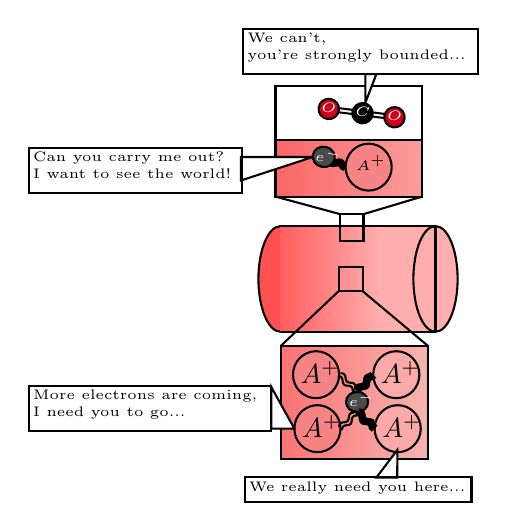
\begin{tikzpicture}[x=0.5pt,y=0.5pt,yscale=-1,xscale=1]
%uncomment if require: \path (0,379); %set diagram left start at 0, and has height of 379

%Shape: Ellipse [id:dp9622117368370047] 
\draw  [color={rgb, 255:red, 0; green, 0; blue, 0 }  ,draw opacity=1 ][fill={rgb, 255:red, 255; green, 81; blue, 81 }  ,fill opacity=1 ] (261,195.83) .. controls (261,174.75) and (268.16,157.67) .. (276.98,157.67) .. controls (285.81,157.67) and (292.97,174.75) .. (292.97,195.83) .. controls (292.97,216.91) and (285.81,234) .. (276.98,234) .. controls (268.16,234) and (261,216.91) .. (261,195.83) -- cycle ;
%Flowchart: Process [id:dp28422413474297636] 
\draw  [draw opacity=0][shading=_cfniglq4v,_gybj19fho] (276.98,157.67) -- (388.98,157.67) -- (388.98,234) -- (276.98,234) -- cycle ;
%Shape: Ellipse [id:dp35622392665186065] 
\draw  [color={rgb, 255:red, 0; green, 0; blue, 0 }  ,draw opacity=1 ][fill={rgb, 255:red, 255; green, 173; blue, 173 }  ,fill opacity=1 ] (373,195.83) .. controls (373,174.75) and (380.16,157.67) .. (388.98,157.67) .. controls (397.81,157.67) and (404.97,174.75) .. (404.97,195.83) .. controls (404.97,216.91) and (397.81,234) .. (388.98,234) .. controls (380.16,234) and (373,216.91) .. (373,195.83) -- cycle ;

%Straight Lines [id:da18690534808046555] 
\draw    (276.98,157.67) -- (388.98,157.67) ;
%Straight Lines [id:da1066274739877433] 
\draw    (388.98,157.67) -- (388.98,234) ;
%Shape: Rectangle [id:dp4433383857974307] 
\draw   (320,149) -- (336.97,149) -- (336.97,168.67) -- (320,168.67) -- cycle ;
%Shape: Rectangle [id:dp7537631586971683] 
\draw  [fill={rgb, 255:red, 255; green, 255; blue, 255 }  ,fill opacity=1 ] (273.33,56.07) -- (379.33,56.07) -- (379.33,96.7) -- (273.33,96.7) -- cycle ;
%Shape: Rectangle [id:dp37218914462590813] 
\path  [shading=_ajm3hcsak,_lo39j7rqb] (273.33,95.7) -- (379.33,95.7) -- (379.33,136.33) -- (273.33,136.33) -- cycle ; % for fading 
 \draw   (273.33,95.7) -- (379.33,95.7) -- (379.33,136.33) -- (273.33,136.33) -- cycle ; % for border 

%Shape: Rectangle [id:dp5470932641139415] 
\draw   (319,187.07) -- (336.33,187.07) -- (336.33,204.67) -- (319,204.67) -- cycle ;
%Straight Lines [id:da6253182506012112] 
\draw    (273.33,136.33) -- (320,149) ;
%Straight Lines [id:da8939419370951256] 
\draw    (379.33,136.33) -- (336.97,149) ;
%Straight Lines [id:da09366117289910447] 
\draw    (276.98,234) -- (388.98,234) ;
%Shape: Rectangle [id:dp8432460991426698] 
\path  [shading=_yinjv7gur,_y44xlpvuy] (277.33,244.07) -- (383.33,244.07) -- (383.33,326.07) -- (277.33,326.07) -- cycle ; % for fading 
 \draw   (277.33,244.07) -- (383.33,244.07) -- (383.33,326.07) -- (277.33,326.07) -- cycle ; % for border 

%Straight Lines [id:da013743908297652263] 
\draw    (383.33,244.07) -- (336.33,204.67) ;
%Straight Lines [id:da14098052123936788] 
\draw    (277.33,244.07) -- (319,204.67) ;
%Shape: Ellipse [id:dp6247211631294155] 
\draw  [fill={rgb, 255:red, 247; green, 132; blue, 132 }  ,fill opacity=1 ] (286,265.03) .. controls (286,255.66) and (293.46,248.07) .. (302.67,248.07) .. controls (311.87,248.07) and (319.33,255.66) .. (319.33,265.03) .. controls (319.33,274.4) and (311.87,282) .. (302.67,282) .. controls (293.46,282) and (286,274.4) .. (286,265.03) -- cycle ;

%Shape: Ellipse [id:dp09933838704347231] 
\draw  [fill={rgb, 255:red, 252; green, 169; blue, 169 }  ,fill opacity=1 ] (344,265.03) .. controls (344,255.66) and (351.46,248.07) .. (360.67,248.07) .. controls (369.87,248.07) and (377.33,255.66) .. (377.33,265.03) .. controls (377.33,274.4) and (369.87,282) .. (360.67,282) .. controls (351.46,282) and (344,274.4) .. (344,265.03) -- cycle ;

%Shape: Ellipse [id:dp23951700441672552] 
\draw  [fill={rgb, 255:red, 74; green, 74; blue, 74 }  ,fill opacity=1 ] (324.33,284.7) .. controls (324.33,280.63) and (327.92,277.33) .. (332.33,277.33) .. controls (336.75,277.33) and (340.33,280.63) .. (340.33,284.7) .. controls (340.33,288.77) and (336.75,292.07) .. (332.33,292.07) .. controls (327.92,292.07) and (324.33,288.77) .. (324.33,284.7) -- cycle ;

%Shape: Ellipse [id:dp6369381811901348] 
\draw  [fill={rgb, 255:red, 252; green, 169; blue, 169 }  ,fill opacity=1 ] (345,304.03) .. controls (345,294.66) and (352.46,287.07) .. (361.67,287.07) .. controls (370.87,287.07) and (378.33,294.66) .. (378.33,304.03) .. controls (378.33,313.4) and (370.87,321) .. (361.67,321) .. controls (352.46,321) and (345,313.4) .. (345,304.03) -- cycle ;

%Shape: Ellipse [id:dp7291394893338838] 
\draw  [fill={rgb, 255:red, 247; green, 132; blue, 132 }  ,fill opacity=1 ] (287,304.03) .. controls (287,294.66) and (294.46,287.07) .. (303.67,287.07) .. controls (312.87,287.07) and (320.33,294.66) .. (320.33,304.03) .. controls (320.33,313.4) and (312.87,321) .. (303.67,321) .. controls (294.46,321) and (287,313.4) .. (287,304.03) -- cycle ;

%Shape: Ellipse [id:dp22227586019609624] 
\draw  [fill={rgb, 255:red, 208; green, 2; blue, 27 }  ,fill opacity=1 ] (304.56,72.05) .. controls (305.07,68.03) and (308.74,65.17) .. (312.77,65.68) .. controls (316.8,66.19) and (319.65,69.87) .. (319.14,73.9) .. controls (318.63,77.93) and (314.96,80.78) .. (310.93,80.27) .. controls (306.9,79.76) and (304.05,76.08) .. (304.56,72.05) -- cycle ;
%Shape: Ellipse [id:dp17169965296099154] 
\draw  [fill={rgb, 255:red, 0; green, 0; blue, 0 }  ,fill opacity=1 ] (328.94,75.14) .. controls (329.45,71.11) and (333.13,68.26) .. (337.16,68.77) .. controls (341.18,69.28) and (344.04,72.96) .. (343.53,76.98) .. controls (343.02,81.01) and (339.34,83.86) .. (335.31,83.35) .. controls (331.28,82.84) and (328.43,79.17) .. (328.94,75.14) -- cycle ;
%Shape: Ellipse [id:dp011360732977615307] 
\draw  [fill={rgb, 255:red, 208; green, 2; blue, 27 }  ,fill opacity=1 ] (352.07,78.06) .. controls (352.58,74.04) and (356.26,71.18) .. (360.29,71.69) .. controls (364.32,72.2) and (367.17,75.88) .. (366.66,79.91) .. controls (366.15,83.94) and (362.47,86.79) .. (358.44,86.28) .. controls (354.41,85.77) and (351.56,82.09) .. (352.07,78.06) -- cycle ;
%Straight Lines [id:da7974115124186444] 
\draw    (319.33,72.41) -- (329.13,73.65)(318.96,75.39) -- (328.75,76.63) ;
%Straight Lines [id:da5182902810935426] 
\draw    (343.71,75.5) -- (352.26,76.58)(343.34,78.47) -- (351.88,79.55) ;
%Shape: Triangle [id:dp39508800979711045] 
\draw  [fill={rgb, 255:red, 255; green, 255; blue, 255 }  ,fill opacity=1 ] (346.28,47.79) -- (338.36,47.77) -- (338.29,68.44) -- cycle ;
%Shape: Ellipse [id:dp15334502924440074] 
\draw  [fill={rgb, 255:red, 247; green, 132; blue, 132 }  ,fill opacity=1 ] (324,115.03) .. controls (324,105.66) and (331.46,98.07) .. (340.67,98.07) .. controls (349.87,98.07) and (357.33,105.66) .. (357.33,115.03) .. controls (357.33,124.4) and (349.87,132) .. (340.67,132) .. controls (331.46,132) and (324,124.4) .. (324,115.03) -- cycle ;
%Shape: Triangle [id:dp6881915358892967] 
\draw  [fill={rgb, 255:red, 255; green, 255; blue, 255 }  ,fill opacity=1 ] (248.33,124.7) -- (248.33,107.7) -- (300.33,107.7) -- cycle ;
%Straight Lines [id:da2622642036826208] 
\draw [line width=1.5]    (308.88,106.25) .. controls (311.1,105.45) and (312.61,106.16) .. (313.4,108.38) .. controls (314.2,110.6) and (315.71,111.31) .. (317.93,110.51) .. controls (320.15,109.71) and (321.66,110.42) .. (322.45,112.64) -- (324.64,113.68) -- (324.64,113.68)(307.6,108.96) .. controls (309.82,108.16) and (311.33,108.87) .. (312.12,111.09) .. controls (312.92,113.31) and (314.43,114.02) .. (316.65,113.23) .. controls (318.87,112.43) and (320.38,113.14) .. (321.17,115.36) -- (323.36,116.39) -- (323.36,116.39) ;
%Shape: Ellipse [id:dp6143309725459223] 
\draw  [fill={rgb, 255:red, 74; green, 74; blue, 74 }  ,fill opacity=1 ] (300.41,105.95) .. controls (301.26,101.97) and (305.44,99.48) .. (309.77,100.4) .. controls (314.09,101.31) and (316.91,105.28) .. (316.07,109.26) .. controls (315.22,113.24) and (311.04,115.73) .. (306.71,114.81) .. controls (302.39,113.9) and (299.57,109.93) .. (300.41,105.95) -- cycle ;

%Straight Lines [id:da9760937342028512] 
\draw [line width=1.5]    (331.25,276.3) .. controls (331.18,273.94) and (332.33,272.73) .. (334.69,272.67) .. controls (337.04,272.61) and (338.19,271.4) .. (338.13,269.05) .. controls (338.07,266.7) and (339.22,265.49) .. (341.57,265.42) -- (342.91,264) -- (342.91,264)(333.42,278.37) .. controls (333.36,276.01) and (334.51,274.8) .. (336.86,274.74) .. controls (339.21,274.67) and (340.36,273.46) .. (340.3,271.11) .. controls (340.24,268.76) and (341.39,267.55) .. (343.74,267.48) -- (345.09,266.07) -- (345.09,266.07) ;
%Straight Lines [id:da5076107925216874] 
\draw [line width=1.5]    (333.36,290.98) .. controls (335.72,290.91) and (336.93,292.06) .. (337,294.41) .. controls (337.07,296.76) and (338.28,297.91) .. (340.63,297.84) .. controls (342.99,297.77) and (344.2,298.92) .. (344.27,301.28) -- (346.03,302.94) -- (346.03,302.94)(331.3,293.16) .. controls (333.66,293.09) and (334.87,294.24) .. (334.94,296.59) .. controls (335.01,298.94) and (336.22,300.09) .. (338.57,300.02) .. controls (340.93,299.95) and (342.14,301.1) .. (342.21,303.46) -- (343.97,305.12) -- (343.97,305.12) ;
%Straight Lines [id:da9783053737580983] 
\draw [line width=0.75]    (320.36,263.94) .. controls (322.72,263.87) and (323.93,265.02) .. (324,267.38) .. controls (324.07,269.73) and (325.28,270.88) .. (327.63,270.82) .. controls (329.98,270.75) and (331.19,271.9) .. (331.26,274.25) -- (333.36,276.24) -- (333.36,276.24)(318.3,266.12) .. controls (320.66,266.06) and (321.87,267.21) .. (321.93,269.56) .. controls (322,271.92) and (323.21,273.07) .. (325.57,273) .. controls (327.92,272.93) and (329.13,274.08) .. (329.2,276.43) -- (331.3,278.42) -- (331.3,278.42) ;
%Straight Lines [id:da4343803839621099] 
\draw [line width=0.75]    (319.27,302.97) .. controls (319.28,300.62) and (320.46,299.44) .. (322.81,299.44) .. controls (325.17,299.45) and (326.35,298.27) .. (326.36,295.91) .. controls (326.36,293.55) and (327.54,292.37) .. (329.9,292.38) -- (331.27,291) -- (331.27,291)(321.39,305.1) .. controls (321.39,302.74) and (322.57,301.56) .. (324.93,301.56) .. controls (327.29,301.57) and (328.47,300.39) .. (328.47,298.03) .. controls (328.47,295.67) and (329.65,294.49) .. (332.01,294.5) -- (333.39,293.13) -- (333.39,293.13) ;
%Shape: Triangle [id:dp9357082470107758] 
\draw  [fill={rgb, 255:red, 255; green, 255; blue, 255 }  ,fill opacity=1 ] (346.26,339.34) -- (361.33,339.4) -- (361.41,319.46) -- cycle ;
%Shape: Triangle [id:dp19117374866461523] 
\draw  [fill={rgb, 255:red, 255; green, 255; blue, 255 }  ,fill opacity=1 ] (270.33,273.97) -- (270.33,304.03) -- (287,304.03) -- cycle ;

% Text Node
\draw (329.7,68.57) node [anchor=north west][inner sep=0.75pt]  [font=\tiny,color={rgb, 255:red, 255; green, 255; blue, 255 }  ,opacity=1 ,rotate=-7.21]  {$C$};
% Text Node
\draw (352.62,71.47) node [anchor=north west][inner sep=0.75pt]  [font=\tiny,color={rgb, 255:red, 255; green, 255; blue, 255 }  ,opacity=1 ,rotate=-7.21]  {$O$};
% Text Node
\draw (305.11,65.46) node [anchor=north west][inner sep=0.75pt]  [font=\tiny,color={rgb, 255:red, 255; green, 255; blue, 255 }  ,opacity=1 ,rotate=-7.21]  {$O$};
% Text Node
\draw (329.33,104.19) node [anchor=north west][inner sep=0.75pt]  [font=\tiny]  {$A^{+}$};
% Text Node
\draw    (250,15) -- (420,15) -- (420,48) -- (250,48) -- cycle  ;
\draw (251,16) node [anchor=north west][inner sep=0.75pt]  [font=\tiny] [align=left] {We can't, \\you're strongly bounded...};
% Text Node
\draw    (95,101) -- (249,101) -- (249,134) -- (95,134) -- cycle  ;
\draw (96,102) node [anchor=north west][inner sep=0.75pt]  [font=\tiny] [align=left] {Can you carry me out? \\I want to see the world!};
% Text Node
\draw    (251,339) -- (415,339) -- (415,357) -- (251,357) -- cycle  ;
\draw (252,340) node [anchor=north west][inner sep=0.75pt]  [font=\tiny] [align=left] {We really need you here...};
% Text Node
\draw    (95,273) -- (270,273) -- (270,306) -- (95,306) -- cycle  ;
\draw (96,274) node [anchor=north west][inner sep=0.75pt]  [font=\tiny] [align=left] {More electrons are coming,\\I need you to go...};
% Text Node
\draw (302.17,96.76) node [anchor=north west][inner sep=0.75pt]  [font=\tiny,color={rgb, 255:red, 255; green, 255; blue, 255 }  ,opacity=1 ,rotate=-11.95]  {$e^{-\ }$};
% Text Node
\draw (290.33,292.19) node [anchor=north west][inner sep=0.75pt]    {$A^{+}$};
% Text Node
\draw (348.33,292.19) node [anchor=north west][inner sep=0.75pt]    {$A^{+}$};
% Text Node
\draw (324.14,275.35) node [anchor=north west][inner sep=0.75pt]  [font=\tiny,color={rgb, 255:red, 255; green, 255; blue, 255 }  ,opacity=1 ]  {$e^{-\ }$};
% Text Node
\draw (347.33,253.19) node [anchor=north west][inner sep=0.75pt]    {$A^{+}$};
% Text Node
\draw (289.33,253.19) node [anchor=north west][inner sep=0.75pt]    {$A^{+}$};


\end{tikzpicture}
\caption{Electrons' behavior in conductor body(bottom inlet) and solid-air interface(top inlet). The wavy lines represent interactions between different particles, and the weight of those lines indicates the interaction strength.}
\label{fig3}
\end{marginfigure}

\begin{equation}
    \dot{Q}_{conv}=h_mA_s(T_s-T_{\infty})
    \label{eqn1}
\end{equation}
with $h_m$ and $A_s$ being "\textbf{convection coefficient}" and surface area, respectively. With Eqn. (\ref{eqn1}), we are now well-equipped to derive another governing equation for the convection and conduction process in a solid by employing the conservation law of thermal energy.

Similar to what we did in Lab1, we cut a thin slice out of an one-dimensional thermal conductor with arbitrary geometry(see Fig.\ref{fig4}). Here we again have some heat flux $q_l$ coming in at the left and some coming out at the right ($q_r$). On the surface, molecules in the air take heat away with a rate of $\dot{Q}_{conv}$. The conservation of energy tells us that the total change in the thermal energy of the slice $\Delta Q$ is simply

\begin{equation}
    \Delta Q=q_lA_{c,l}dt-q_rA_{c,r}dt-\dot{Q}_{conv}dt,\label{eqn2}
\end{equation}
where $A_{c,l}$ and $A_{c,r}$ are the cross section areas at left and right faces of the slice, respectively. Recall that, from Lab2, the change in thermal energy $\Delta Q$ is related to \textbf{the change in temperature} $T_l-T_r$ by the following equation:

\begin{equation}
    \Delta Q=mc_p(T_l-T_r)
\end{equation}

\begin{marginfigure}
% Gradient Info
\tikzset {_oliva5ufb/.code = {\pgfsetadditionalshadetransform{ \pgftransformshift{\pgfpoint{0 bp } { 0 bp }  }  \pgftransformrotate{0 }  \pgftransformscale{2 }  }}}
\pgfdeclarehorizontalshading{_5u6e74wx5}{150bp}{rgb(0bp)=(0.98,0.24,0.24);
rgb(37.5bp)=(0.98,0.24,0.24);
rgb(62.5bp)=(0.98,0.53,0.53);
rgb(100bp)=(0.98,0.53,0.53)}

% Gradient Info
\tikzset {_wmyan5znt/.code = {\pgfsetadditionalshadetransform{ \pgftransformshift{\pgfpoint{0 bp } { 0 bp }  }  \pgftransformrotate{0 }  \pgftransformscale{2 }  }}}
\pgfdeclarehorizontalshading{_vfd3yyfvx}{150bp}{rgb(0bp)=(0.98,0.24,0.24);
rgb(37.5bp)=(0.98,0.24,0.24);
rgb(62.5bp)=(0.98,0.53,0.53);
rgb(100bp)=(0.98,0.53,0.53)}

% Gradient Info
\tikzset {_bmzdjp8dp/.code = {\pgfsetadditionalshadetransform{ \pgftransformshift{\pgfpoint{0 bp } { 0 bp }  }  \pgftransformrotate{0 }  \pgftransformscale{2 }  }}}
\pgfdeclarehorizontalshading{_bf0lhynp4}{150bp}{rgb(0bp)=(0.98,0.24,0.24);
rgb(37.5bp)=(0.98,0.24,0.24);
rgb(62.5bp)=(0.98,0.53,0.53);
rgb(100bp)=(0.98,0.53,0.53)}
\tikzset{every picture/.style={line width=0.75pt}} %set default line width to 0.75pt        
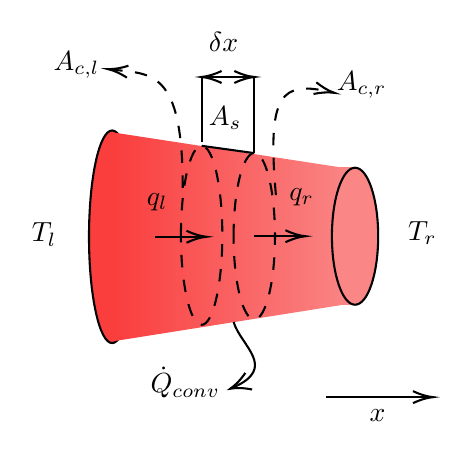
\begin{tikzpicture}[x=0.66pt,y=0.66pt,yscale=-1,xscale=1]
%uncomment if require: \path (0,300); %set diagram left start at 0, and has height of 300

%Shape: Ellipse [id:dp0992860075306039] 
\draw  [fill={rgb, 255:red, 250; green, 61; blue, 61 }  ,fill opacity=1 ] (174,138.2) .. controls (174,106.06) and (179.67,80) .. (186.67,80) .. controls (193.66,80) and (199.33,106.06) .. (199.33,138.2) .. controls (199.33,170.34) and (193.66,196.4) .. (186.67,196.4) .. controls (179.67,196.4) and (174,170.34) .. (174,138.2) -- cycle ;
%Shape: Triangle [id:dp11747064853141964] 
\draw  [draw opacity=0][shading=_5u6e74wx5,_oliva5ufb] (186.67,81) -- (319.67,101.4) -- (186.67,101.4) -- cycle ;
%Shape: Triangle [id:dp6083398190383781] 
\draw  [draw opacity=0][shading=_vfd3yyfvx,_wmyan5znt] (187.33,195.4) -- (319.67,174.4) -- (186.67,174.4) -- cycle ;
%Shape: Rectangle [id:dp22173112935264783] 
\draw  [draw opacity=0][shading=_bf0lhynp4,_bmzdjp8dp] (186.67,100.4) -- (319.67,100.4) -- (319.67,175.4) -- (186.67,175.4) -- cycle ;
%Shape: Ellipse [id:dp38588778333343166] 
\draw  [fill={rgb, 255:red, 251; green, 134; blue, 134 }  ,fill opacity=1 ] (307,137.9) .. controls (307,117.19) and (312.67,100.4) .. (319.67,100.4) .. controls (326.66,100.4) and (332.33,117.19) .. (332.33,137.9) .. controls (332.33,158.61) and (326.66,175.4) .. (319.67,175.4) .. controls (312.67,175.4) and (307,158.61) .. (307,137.9) -- cycle ;
%Shape: Ellipse [id:dp3301273323477486] 
\draw  [dash pattern={on 4.5pt off 4.5pt}] (224.33,137.4) .. controls (224.33,110.34) and (229.41,88.4) .. (235.67,88.4) .. controls (241.93,88.4) and (247,110.34) .. (247,137.4) .. controls (247,164.46) and (241.93,186.4) .. (235.67,186.4) .. controls (229.41,186.4) and (224.33,164.46) .. (224.33,137.4) -- cycle ;
%Shape: Ellipse [id:dp5079826231310873] 
\draw  [dash pattern={on 4.5pt off 4.5pt}] (253.17,137.9) .. controls (253.17,112.77) and (258.24,92.4) .. (264.5,92.4) .. controls (270.76,92.4) and (275.83,112.77) .. (275.83,137.9) .. controls (275.83,163.03) and (270.76,183.4) .. (264.5,183.4) .. controls (258.24,183.4) and (253.17,163.03) .. (253.17,137.9) -- cycle ;
%Straight Lines [id:da4637457686436022] 
\draw    (235.67,86.45) -- (235.67,50.72) ;
%Straight Lines [id:da14588683949865355] 
\draw    (264.5,92.4) -- (264.5,50.72) ;
%Straight Lines [id:da6084736749348655] 
\draw    (237.67,50.72) -- (262.5,50.72) ;
\draw [shift={(264.5,50.72)}, rotate = 180] [color={rgb, 255:red, 0; green, 0; blue, 0 }  ][line width=0.75]    (10.93,-3.29) .. controls (6.95,-1.4) and (3.31,-0.3) .. (0,0) .. controls (3.31,0.3) and (6.95,1.4) .. (10.93,3.29)   ;
\draw [shift={(235.67,50.72)}, rotate = 0] [color={rgb, 255:red, 0; green, 0; blue, 0 }  ][line width=0.75]    (10.93,-3.29) .. controls (6.95,-1.4) and (3.31,-0.3) .. (0,0) .. controls (3.31,0.3) and (6.95,1.4) .. (10.93,3.29)   ;
%Straight Lines [id:da5783371827872952] 
\draw    (210.33,138.2) -- (236.33,138.2) ;
\draw [shift={(238.33,138.2)}, rotate = 180] [color={rgb, 255:red, 0; green, 0; blue, 0 }  ][line width=0.75]    (10.93,-3.29) .. controls (6.95,-1.4) and (3.31,-0.3) .. (0,0) .. controls (3.31,0.3) and (6.95,1.4) .. (10.93,3.29)   ;
%Straight Lines [id:da36299192344581266] 
\draw    (264.5,137.9) -- (290.5,137.9) ;
\draw [shift={(292.5,137.9)}, rotate = 180] [color={rgb, 255:red, 0; green, 0; blue, 0 }  ][line width=0.75]    (10.93,-3.29) .. controls (6.95,-1.4) and (3.31,-0.3) .. (0,0) .. controls (3.31,0.3) and (6.95,1.4) .. (10.93,3.29)   ;
%Curve Lines [id:da8671908755206263] 
\draw    (253.17,184.9) .. controls (257.25,198.13) and (277.5,209.92) .. (252.9,220.74) ;
\draw [shift={(251.33,221.4)}, rotate = 337.83000000000004] [color={rgb, 255:red, 0; green, 0; blue, 0 }  ][line width=0.75]    (10.93,-4.9) .. controls (6.95,-2.3) and (3.31,-0.67) .. (0,0) .. controls (3.31,0.67) and (6.95,2.3) .. (10.93,4.9)   ;
%Curve Lines [id:da49512178175313826] 
\draw  [dash pattern={on 4.5pt off 4.5pt}]  (225.33,111.4) .. controls (225.33,46.07) and (208.22,49.19) .. (186.05,46.61) ;
\draw [shift={(184.33,46.4)}, rotate = 367.43] [color={rgb, 255:red, 0; green, 0; blue, 0 }  ][line width=0.75]    (10.93,-3.29) .. controls (6.95,-1.4) and (3.31,-0.3) .. (0,0) .. controls (3.31,0.3) and (6.95,1.4) .. (10.93,3.29)   ;
%Curve Lines [id:da03315232539524782] 
\draw  [dash pattern={on 4.5pt off 4.5pt}]  (276.33,115.4) .. controls (271.43,59.54) and (279.02,52.66) .. (306.62,59) ;
\draw [shift={(308.33,59.4)}, rotate = 193.57] [color={rgb, 255:red, 0; green, 0; blue, 0 }  ][line width=0.75]    (10.93,-3.29) .. controls (6.95,-1.4) and (3.31,-0.3) .. (0,0) .. controls (3.31,0.3) and (6.95,1.4) .. (10.93,3.29)   ;
%Straight Lines [id:da33392437202493264] 
\draw    (235.67,88.4) -- (264.5,92.4) ;
%Straight Lines [id:da3400156752874589] 
\draw    (304,226) -- (360.33,226) ;
\draw [shift={(362.33,226)}, rotate = 180] [color={rgb, 255:red, 0; green, 0; blue, 0 }  ][line width=0.75]    (10.93,-3.29) .. controls (6.95,-1.4) and (3.31,-0.3) .. (0,0) .. controls (3.31,0.3) and (6.95,1.4) .. (10.93,3.29)   ;

% Text Node
\draw (238,24.29) node [anchor=north west][inner sep=0.75pt]    {$\delta x$};
% Text Node
\draw (204,113) node [anchor=north west][inner sep=0.75pt]    {$q_{l}$};
% Text Node
\draw (282,110) node [anchor=north west][inner sep=0.75pt]    {$q_{r}$};
% Text Node
\draw (206,208) node [anchor=north west][inner sep=0.75pt]    {$\dot{Q}_{conv}$};
% Text Node
\draw (153,35) node [anchor=north west][inner sep=0.75pt]    {$A_{c,l}$};
% Text Node
\draw (308,46) node [anchor=north west][inner sep=0.75pt]    {$A_{c,r}$};
% Text Node
\draw (238,65) node [anchor=north west][inner sep=0.75pt]    {$A_{s}$};
% Text Node
\draw (141,129) node [anchor=north west][inner sep=0.75pt]    {$T_{l}$};
% Text Node
\draw (347,128) node [anchor=north west][inner sep=0.75pt]    {$T_{r}$};
% Text Node
\draw (326,231) node [anchor=north west][inner sep=0.75pt]    {$x$};


\end{tikzpicture}
\caption{A slice of conductor with non-uniform cross section}
\label{fig4}
\end{marginfigure}
\noindent where the mass of the slice is $m=\rho\int_0^{\delta x} A_c(x)dx$ with $\delta x$ being slice thickness. We now write $\dot{Q}_{conv}$ explicitly using Eqn.(\ref{eqn1}), and divide both sides of Eqn. (\ref{eqn2}) by $dt$ to give

\begin{equation}
    \rho\int_0^{\delta} A_c(x)dx\frac{\partial T}{\partial t}=q_lA_{c,l}-q_rA_{c,r}-h_mA_s(T-T_{\infty}).
    \label{eqn3}
\end{equation}

Eqn.\ref{eqn3} implies two assumptions: \imp{(1) the change in temperature is one-dimensional so the surface temperature is equal to the body temperature, and (2) the change in temperature is negligible at the slice outer surface(i.e. $T$ is not a function of $x$ at surface)}. With these assumptions, we now take a first derivative with respect to $x$ at both sides of Eqn.\ref{eqn3} to give

\begin{equation}
    \rho A_c(x)\frac{\partial T}{\partial t}=-\frac{\partial (qA_c)}{\partial x}-h_m\frac{d A_s}{dx}(T-T_{\infty}).
\end{equation}

Once again, we can derive a governing equation free of flux $q$ by applying \textbf{Fourier's law} to give

\begin{equation}
    \rho A_c(x)\frac{\partial T}{\partial t}=-\frac{\partial }{\partial x}\left(-\kappa\frac{\partial T}{\partial x}A_c\right)-h_m\frac{d A_s}{dx}(T-T_{\infty}).
    \label{eqn6}
\end{equation}
Eqn.\ref{eqn6} is the so-called \imp{heat equation for extended surface}\index{heat equation for extended surface}.

Newton's cooling law gives the macroscopic description of convection. At atomic level, the molecules in the air collide with the hot surface while taking some energy off the solid through the process of elastic collision\footnote{\href{https://en.wikipedia.org/wiki/Elastic_collision}{Elastic collision on Wikipedia}}. But it was not long after John Tyndall\footnote{\href{https://en.wikipedia.org/wiki/John_Tyndall}{John Tyndall on Wikipedia}} showed his fellow scientists how to measure infrared emission from a platinum filament, people started to wondering whether Eqn.(\ref{eqn1}) is still valid as there is one more mechanism for interfacial heat transfer except convection, that is, thermal radiation.

\subsection{Buoyancy: things happen to heated molecules}

\quad Before we discuss radiative heat transfer, there are something about the heated air worth mentioning. Why do we care about what happen to them? The answer to this question helps us to understand the concept of \textbf{buoyancy}, which is a key fluid property to engineers when they want to design a proper cooling system for large infrastructures such as internet server farm. After one or multiple collisions, ambient molecules take thermal energy off the solid surface, which adds to their kinetic energies. Those hot molecules have a tendency of fast moving in the ambient environment, and travel longer distances than those cold molecules. \textbf{At macroscopic level, a large group of hot gas molecules expands in the ambient environment, resulting in decreased density.} Now imagine that the hot air is contained in a mass-less but thermally insulating balloon which allows the hot air to expand freely.\footnote{In the real world, the pressure inside a balloon is always slightly higher than the pressure outside of the balloon. This phonomenon is described by the \href{https://en.wikipedia.org/wiki/Young\%E2\%80\%93Laplace_equation}{\textbf{Young–Laplace equation}}} According to Archimedes' principle, the cold air applies an upward force to the balloon, $F_b$, and

\begin{equation}
    F_b=-\rho_{cold} g V
    \label{eqn7}
\end{equation}
with $\rho_{cold}$ and $V$ being the density of cold air and the balloon volume in our case. Because the density of hot air, $\rho_{hot}$, is less than $\rho_{cold}$, $F_b$ is larger than the gravity of hot air. Without any influence of wind, the mass-less balloon should float upwards until it reaches an altitude where $\rho_{cold}=\rho_{hot}$. \footnote{In the reality, hot air balloons are operating upon the similar principle. A fun fact about commercial balloons is that one cubic meter air is able to drag a mass of 7grams when it is heated to 100${}^oF$.}

Knowing the buoyancy of hot air can help us to see why natural convection is not an efficient way to dissipate heat in large-scale infrastructure. From Eqn. (\ref{eqn1}) the convective heat transfer rate depends on temperature difference between the heated body and its surrounding. However, the heated air near the bottom of a large body will float upwards to the top where the temperature difference is no longer large because of the accumulation of hot air. As a result, the upper part of the body will be overheating. For a large-scale electronic infrastructure, overheating is the primary killer of device health. To avoid this problem, engineers have designed various forced cooling methods, such as water cooling and fan cooling. 
\begin{marginfigure}[0.0in]
% Gradient Info
\tikzset {_744lsv54u/.code = {\pgfsetadditionalshadetransform{ \pgftransformshift{\pgfpoint{0 bp } { 0 bp }  }  \pgftransformrotate{0 }  \pgftransformscale{2 }  }}}
\pgfdeclarehorizontalshading{_at5uudijf}{150bp}{rgb(0bp)=(1,0.22,0.22);
rgb(37.5bp)=(1,0.22,0.22);
rgb(62.5bp)=(1,0.65,0.65);
rgb(100bp)=(1,0.65,0.65)}
\tikzset{every picture/.style={line width=0.75pt}} %set default line width to 0.75pt        
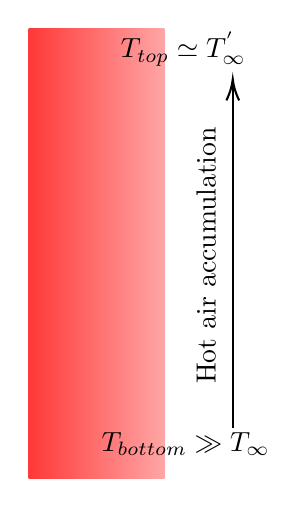
\begin{tikzpicture}[x=0.7pt,y=0.7pt,yscale=-1,xscale=1]
%uncomment if require: \path (0,300); %set diagram left start at 0, and has height of 300

%Shape: Rectangle [id:dp5006565224455771] 
\draw  [draw opacity=0][shading=_at5uudijf,_744lsv54u] (454,33.07) -- (524,33.07) -- (524,265.07) -- (454,265.07) -- cycle ;
%Straight Lines [id:da590769886276838] 
\draw    (559.33,239.07) -- (559.33,61.07) ;
\draw [shift={(559.33,59.07)}, rotate = 450] [color={rgb, 255:red, 0; green, 0; blue, 0 }  ][line width=0.75]    (10.93,-3.29) .. controls (6.95,-1.4) and (3.31,-0.3) .. (0,0) .. controls (3.31,0.3) and (6.95,1.4) .. (10.93,3.29)   ;


% Text Node
\draw (539,218) node [anchor=north west][inner sep=0.75pt]  [rotate=-270] [align=left] {Hot air accumulation};
% Text Node
\draw (500,33) node [anchor=north west][inner sep=0.75pt]    {$T_{top} \simeq T^{'}_{\infty }$};
% Text Node
\draw (490,240) node [anchor=north west][inner sep=0.75pt]    {$T_{bottom} \gg T_{\infty }$};
\end{tikzpicture}
\caption{Hot air accumulation due to the buoyancy}
\label{fig5}
\end{marginfigure}
 

\section{A Few Words on Radiation}
\quad Radiation is perhaps the most special one among the three primary heat transfer mechanisms as it relies on neither solid nor fluid to transport heat. Instead, it is the electromagnetic wave that carries thermal energy and gets emitted or absorbed at surface of solids. People postulate the effects of radiation of visible light since ancient farming society without knowing its electromagnetic nature. Then, in 1888, German physicist \textbf{Heinrich Hertz} succeeded in demonstrating the existence of long-wavelength electromagnetic waves and showed that their properties are consistent with those of the shorter-wavelength visible light\footnote{\href{https://www.britannica.com/science/light/Light-as-electromagnetic-radiation}{Light as electromagnetic radiation on Britannica}}. Two decades before that, \textbf{James Maxwell}, in his formalation of electromagnetism, describes light as a propagating wave of electromagnetic fields, from which he predicted the existence of electromagnetic radiation.

In the case of heat transfer by thermal radiation, \imp{we can write radiative heat flux $q_{rad}$ using a form similar to Newton's cooling law(see Eq.(\ref{eqn8})).} People rely on this formalism because the mean heat transfer coefficient $h_m$ can then be written as a sum of convective $h_{m,c}$ and radiative coefficients $h_{m,r}$(see Eq.(\ref{eqn9})). 
\begin{equation}
    q_{rad}=h_{m,r}(T_s-T_{\infty})
    \label{eqn8}
\end{equation}
\begin{equation}
    q = q_{conv}+q_{rad}=(h_{m,c}+h_{m,r})(T_s-T_{\infty})=h_m(T_s-T_{\infty})
    \label{eqn9}
\end{equation}
As a result, Eqn.(\ref{eqn6}) is still the governing equation for convective+radiative heat transfer process at the heated surface. To get an explicit expression for $h_{m,r}$, we resort to the Stefan-Boltzmann law in which the heat transfer rate varies as the difference in the 4th powers of temperature of solid surface and of ambient environment. In mathematical terms, the radiative heat flux $q_{rad}$ is
\begin{equation}
q_{rad}=\xi \sigma F \left(T_s^{4}-T_{\infty}^{4}\right)
\label{eqn10}
\end{equation}
where $\xi$ is the emissivity\index{emissivity} of the object, $F$ is the so-called "view factor"\index{view factor}, and Stefan-Boltzmann constant\index{Stefan-Boltzmann constant} $\sigma=5.6703 \times 10^{-8}watt/ \mathrm{m}^{2} \mathrm{~K}^{4}$\footnote{$\xi=1$ for black body and $\xi=0.95$ for the coated surface in our experiment, and the view factor $F = 1$.}. We expand the RHS of Eq.(\ref{eqn10}) to give
\begin{equation}
    q_{rad}=\xi\sigma F(T_s+T_{\infty})(T^2_s+T^2_{\infty})(T_s-T_{\infty}).
    \label{eqn11}
\end{equation}
From Eq.(\ref{eqn11}), the "\imp{radiative heat transer coefficient}"\index{radiative heat transfer coefficient} is then
\begin{equation}
    h_{m,r}=\xi\sigma F(T_s+T_{\infty})(T_s^2+T_{\infty}^2).
    \label{eqn12}
\end{equation}
By taking a closer look at Eq.(\ref{eqn12}), we notice that $h_{m,r}$ heavily depents on $T_s$ and $T_{\infty}$, and can not be treated as a constant if significant variation of those temperatures exist in the system. Based on this, people argued that Eq.(\ref{eqn8}) is only valid when the temperature on solid surface is moderately different from ambient temperature, and the surface should be well separated from other surfaces in the system\footnote{Researchers have found that the evanescent waves generated by the reflection of electromagnetic waves inside matters also promote the rate of heat transfer between two surfaces separated only by a small gap, \href{https://pubs.acs.org/doi/10.1021/acsphotonics.8b01031}{see Fig. 1 in this 2018 paper here}}.

\section{Juice from the History}
\quad According to Nikola Tesla, energy, frequency, and vibration tell the secrets of our universe. However, the concept of energy was not well-understood by the scientific community untill 19th century. Before that, age-defining genius such as Isaac Newton, was even afraid of admitting that "temperature" and "heat" are two different things. In his anonymously published paper, \textbf{"Scala graduum Caloris. Calorum Descriptiones \& signa"}, Newton used a small font size at the end to give the first description of the so-called \textbf{Newton's cooling law}\footnote{Newton's law is recently verified by two Japanese researchers using IR camera, and they found Newton's results were “quite accurate”.(\url{https://doi.org/10.1016/j.ijheatmasstransfer.2020.120544}))}, where he argued that the amount of heat getting off solid surface is due to the difference in "\textbf{temperature}", not "\textbf{heat}", between the surface and the environment. Standing at the frontline of mordern physical science, the situation that we're facing now is almost identical to what Newton encountered during his time. Mordern-time physcists argue that our classical world is essentially quantum-mechanical and stochastic at atomistic level. So they believe there must exist an ultimate unification between quantum mechanics and general relativity, with the later describing phenomena at length scale of galaxies. Will scientists find that quantum mechanics and general relativity might be indeed two distinct things just like how we distinguish "heat" from "temperature"? Only the future can tell. For now, let's just worry about things from Newton's time.